\documentclass{beamer}

\usepackage[T1]{fontenc}
\usepackage[utf8]{inputenc}
\usepackage[frenchb]{babel}
\usepackage{eurosym}

\usepackage{graphicx}

% --------- BEGIN STYLE BEAMER ---------
\usetheme{Madrid}
\definecolor{ECNBleu}{HTML}{102648}
\definecolor{ECNJaune}{HTML}{FAB600}

\setbeamercolor{frametitle}{bg=ECNBleu,fg=white} %le titre de la frame, en haut
\setbeamercolor{title in head/foot}{bg=ECNJaune,fg=ECNBleu} %barre bas, milieu
\setbeamercolor{author in head/foot}{bg=ECNBleu,fg=ECNJaune} %barre bas, gauche
\setbeamercolor{date in head/foot}{bg=ECNBleu,fg=ECNJaune} %barre bas, droit
\setbeamercolor{section in head/foot}{bg=ECNJaune,fg=ECNBleu} %haut gauche
\setbeamercolor{subsection in head/foot}{bg=ECNBleu,fg=ECNBleu} %haut droite
\setbeamercolor{title}{bg=ECNBleu,fg=white}
\setbeamercolor{block title}{fg=white,bg=ECNBleu}

%\setbeamercolor{normal text}{bg=IUTBleuFonce} %texte
\setbeamercolor{item}{bg=ECNBleu}
\setbeamercolor{subitem}{bg=ECNJaune}
\setbeamercolor{description item}{fg=couleurEmph}
\setbeamercolor{section in toc}{fg=ECNBleu}
%\setbeamercolor{subsubitem}{bg=IUTBleuFonce}

%structure (eq emph dans beamer)
\setbeamercolor{emph}{fg=couleurEmph}
% ----------------------------

\usepackage{listings}

\lstdefinestyle{customc}{
  belowcaptionskip=1\baselineskip,
  breaklines=true,
  frame=L,
  xleftmargin=\parindent,
  language=C,
  showstringspaces=false,
  basicstyle=\tiny\ttfamily,
  keywordstyle=\bfseries\color{green!40!black},
  commentstyle=\itshape\color{purple!40!black},
  identifierstyle=\color{blue},
  stringstyle=\color{orange},
}

\lstset{escapechar=@,style=customc}

\newenvironment<>{questionblock}[1]{%
\setbeamercolor{block title}{bg=ECNJaune,fg=ECNBleu}%
\begin{block}#2{#1}}{\end{block}}

\title[GPGPU]{Programmation sur Processeur Graphique}
\subtitle[\ldots]{---\\Part 0: séquencement, acquis d'apprentissage et références}
\author[P.-E. Hladik]{Pierre-Emmanuel Hladik\\\tiny pierre-emmanuel.hladik@ec-nantes.fr}
\institute[Centrale Nantes]{}
%{\tiny\date{\today}}
%\logo{
\titlegraphic{
	\flushleft
\includegraphics[width=3cm]{./LogoCN_RVB}
}

\begin{document}

 \frame{\titlepage}
 
 %%%%%%%%%%%%%%%%%%%%%%%%%%%
\section*{Organisation de l'enseignement}
%%%%%%%%%%%%%%%%%%%%%%%%%%%

%%%%%%%%%%%%%%%%%%%%%%%%%%%
\begin{frame}[plain]
\frametitle{Acquis d'apprentissage}

\begin{block}{}
À la fin de cet enseignement l'étudiant :
\begin{itemize}
	\item  connaîtra et saura appliquer les principes de la programmation sur processeurs graphiques (GPU) pour accélérer et optimiser des calculs,
	\item sera capable d’implémenter des algorithmes parallèles en prenant en considération la localité de la mémoire et des données ainsi que les spécificités matérielles du flot de contrôle sur les GPU,
	\item saura implémenter, valider et évaluer les algorithmes classiques de la programmation parallèle afin d’en optimiser les performances.
\end{itemize}
\end{block}

\end{frame}
%%%%%%%%%%%%%%%%%%%%%%%%%%%
\begin{frame}[plain]
\frametitle{Organisation de l'enseignement}

\begin{block}{Séquence}
\begin{enumerate}
	\item Généralités sur la programmation sur GPU
	\begin{itemize}
		\item programmation concurrente vs parallèle
		\item principe et architecture des GPU
	\end{itemize}
	\item Opérateurs, mémoires et structurations des données
	\begin{itemize}
		\item allocation des données et flot de contrôle
		\item types de mémoire et localité des données
		\item opérations atomiques et synchronisation
	\end{itemize}
	\item Etude de patterns d’algorithme pour la programmation parallèles
	\item Exemple d’application : coder un réseau de neurones artificiels
\end{enumerate}
\end{block}

\end{frame}
%%%%%%%%%%%%%%%%%%%%%%%%%%%
\begin{frame}[plain]
\frametitle{Evaluation}

\begin{block}{}
\begin{itemize}
	\item Micro projet individuel (12h TP)
	\item QCM individuel
\end{itemize}
\end{block}

\end{frame}

%%%%%%%%%%%%%%%%%%%%%%%%%%%
\begin{frame}[plain]
\frametitle{Documents de cours}

\center

\includegraphics[width=3cm]{./figures-pdf/qrcode}

\href{https://gitlab.univ-nantes.fr/hladik-pe-1/ecn-gpu-cours}{https://gitlab.univ-nantes.fr/hladik-pe-1/ecn-gpu-cours}


\end{frame}

%%%%%%%%%%%%%%%%%%%%%%%%%%%
\begin{frame}[plain]
\frametitle{Références}
\frametitle{Références}
\begin{columns}[t]
  \begin{column}{0.45\textwidth}
    \begin{block}{Programming Massively Parallel Processors }
    	{\tiny 3rd~Edition: A Hands-on Approach\\
{\bf Auteurs :} David Kirk et Wen-mei W. Hwu}
    \begin{center}
	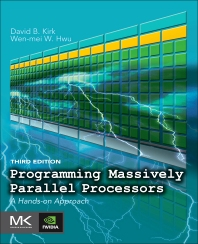
\includegraphics[scale=1]{./figures-pdf/couv_pmpp}
    \end{center}	
	{\tiny 
{\bf O'Reilly Online:} \url{https://cutt.ly/HhQIOGo}\\

{\bf Avis :} très complet et détaillé, une référence dans le domaine.\\
}
	  \end{block}   
  \end{column}
  
  \begin{column}{0.45\textwidth}
    \begin{block}{CUDA by Example}
    	{\tiny 
An Introduction to General-Purpose GPU Programming\\
{\bf Auteurs :} Jason Sanders et Edward Kandrot}
    \begin{center}
	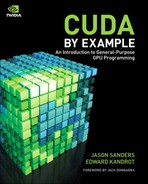
\includegraphics[scale=0.51]{./figures-pdf/couv_cudabyexample}
    \end{center}	
	{\tiny 
{\bf O'Reilly Online:} \url{https://cutt.ly/BhQI9DQ}

{\bf Avis :} introduction efficace et pratique à la programmation avec CUDA.\\
}
	  \end{block}   
  \end{column}
 \end{columns}  
 
     \begin{block}{Nvidia Online training}
{\tiny      \url{https://www.nvidia.com/en-us/deep-learning-ai/education/}}
         \end{block}

\end{frame}
%%%%%%%%%%%%%%%%%%%%%%%%%%

%%%%%%%%%%%%%%%%%%%%%%%%%%%%
%%%%%%%%%%%%%%%%%%%%%%%%%%%%
%\section{Introduction à la programmation parallèle}
%\section{Allocation des données et exécution d'un kernel}
%\section{Kernel à plusieurs dimensions}
%\section{to be continued}
%%%%%%%%%%%%%%%%%%%%%%%%%%%%
%\begin{frame}{Plan}
%\tableofcontents[sections={1-4}]
%\end{frame}
%%%%%%%%%%%%%%%%%%%%%%%%%%%%


\end{document}